\chapter{绪论}
\label{chap:introduction}

\section{领域现状}
随着电子病历系统在医疗机构的迅速普及,大量医疗相关的重要信息以电子形式存储于医疗信息系统中。经过不断积累,各种形式的电子化医疗系统产生了体量庞大的医疗大数据。这些数据记录了临床医疗中的重要信息,例如,病人的主诉,检测结果,诊断信息,服用药物,以及不良反应等。研究人员通过对大量的诊疗数据进行深度分析能够得到与医疗质量与安全、药物疗效等有关的各项指标,根据这些指标可以有针对性的改善医疗质量和效率,同时对于新药物的研发也有着促进作用。根据麦肯锡发布的全球医疗机构分析报告,到2020年,医疗大数据分析市场将为全球节约1900亿美元。

据计生委公布的数据,仅2014年,全国诊疗量就已达到78亿人次。虽然我国的医疗数据电子化进程在近些年来大大加快,不少医院仍然采用纸质病历系统;同时,很多医院也保留着病历系统电子化之前的病历数据。然而,一方面这些纸质化病历数据,数量庞大,不仅在存放和分类管理上需要耗费大量的人力物力,而且也很难与电子化病历系统协同;另一方面,医院内部也有可能有着新旧两套电子病历系统,怎么将旧系统的病历数据迅速迁移到新系统,也是一个不小的挑战。

纸质病历或旧电子病历系统的数据,如果采用人工录入的方式,工程量巨大,录入速度慢,成本也太高。一个可能的解决方案就是采用光学字符识别来采集录入这些病历数据。

\section{光学字符识别}
光学字符识别(Optical Character Recognition,OCR)是指将图片中的字符,翻译成计算机文字的过程\citep{mori1992historical}。
而对于常见的印刷体字符,通过一些光学字符识别软件,将图片中的字符转换成文本格式,这样就可以利用文字处理的软件进行进一步的加工、归档等工作。
对于光学字符识别来说,衡量其性能好坏的几大指标有识别率、识别速度、稳定性、易用性等,其中如何借助一些出错方法和上下文信息提高文字识别的准确率,一直是领域内的重要研究课题。

而对于中文字符识别(Chinese Character Recoginition,CCR),则要比英文字符识别困难许多。
最早的汉字字符识别研究工作可以追溯到1966年,当时IBM公司首先实现了一个能识别1000个汉字的解决方案。
国内的汉字字符识别相关研究开展稍晚,最早开始于70年代末\citep{trier1996feature},之后取得了长足的进步\citep{FanxiaGuo,LongDing}。

\subsection{技术介绍}
光学字符识别是模式识别技术在分类问题上的一个应用。这一类模式识别技术通过从训练数据中提取特征来训练和优化一个分类器,分类器训练完成之后,当有新的数据(测试数据)作为输入时,分类器会给出该输入数据的预测类标。一般来说,训练数据越多,分类器的分类效果就越好。一个典型的OCR系统大致由数据预处理、特征提取、分类器、数据后处理几个部分组成:
\begin{itemize}
	\item 数据预处理:对输入的图像进行处理,突出有用的信息(例如文字),过滤掉无用的背景图片等,以便更好的进行特征提取,在这一步通常的处理方式有:灰度化、二值化、字符切分、倾斜矫正等步骤。
	\item 特征提取:对要识别的文字,我们要提取出可学习的特征,这些特征要使得不同文字在特征空间中的距离尽量大,加大文字间的区分度,常见的特征提取步骤是将处理后的图像数据向量化,并视情况选择是否需要降维。
	\item 分类器:特征提取后的数据需要交给分类器来训练和识别,一般需要一定大小的有标记的数据作为训练样本,对分类器进行训练,比较成熟和常用的分类器有支持向量机(SVM),K近邻,神经网络等。
	\item 数据后处理:分类器识别出来的字符可能并不完全准确,可能需要一些语言模型,利用上下文信息来进行校正。同时,后处理模块还需要对识别的文字进行格式化操作,并且能够正确地被归档,存储到相应的文件中。
\end{itemize}
从上面的描述中,我们可以大致得到一个字符识别的流程图(\autoref{pic:ocr-pipeline}),有关光学字符识别更深入的内容,我们会在\autoref{chap:implements}中详细阐述。

\begin{figure}
\centering
  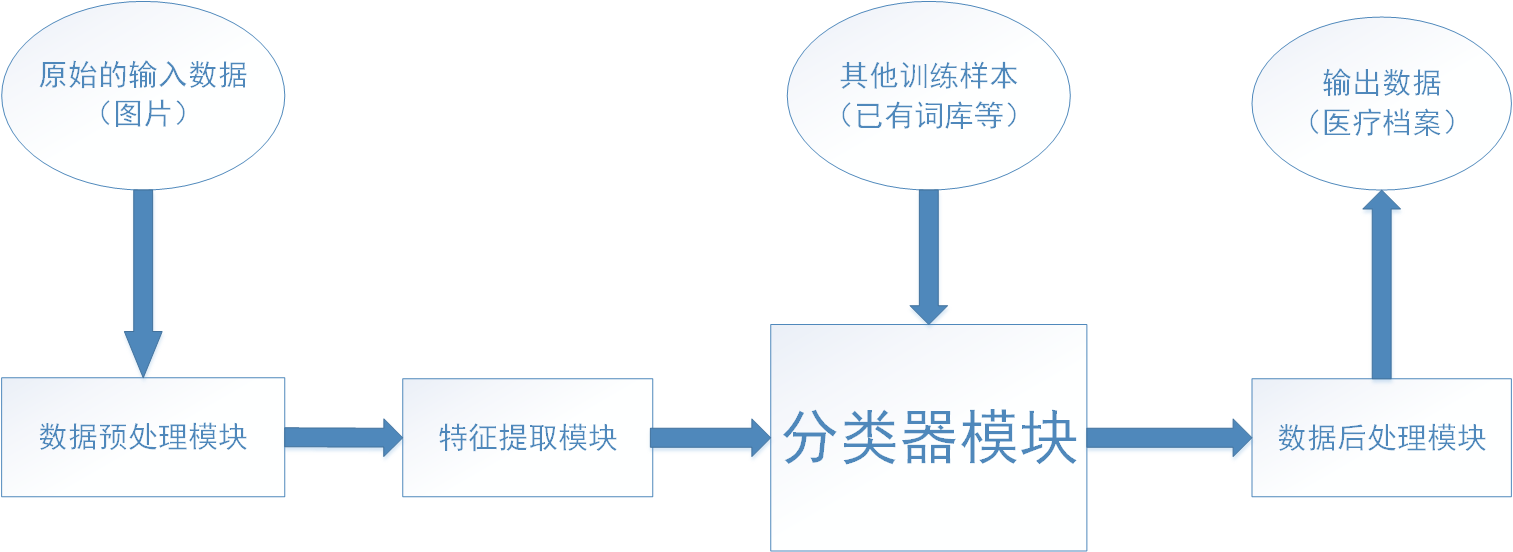
\includegraphics[scale=0.3]{figures/ocr-pipeline}
  \figcaption{光学字符识别系统的整体流程图}
  \label{pic:ocr-pipeline}
\end{figure}

\subsection{应用现状}
近几年国内对印刷体汉字识别的研究不断深入,识别准确率不断上升,也有一些较成熟的商业化产品,比较知名的有泰比(ABBYY)、中文紫光OCR、CAJViewer、清华OCR、尚书七号等。其中尤以泰比的OCR效果为佳,不仅产品线丰富、支持语言多、识别精度高,且对一些表格、框图等复杂数据有比较好的分析能力。但是,购买泰比的OCR服务是昂贵的,仅个人用户使用的专业版就售价1500元之巨,遑论针对企业用户的价格了。除了价格因素外,将现有的商业OCR系统应用到病历数据录入时,一个更棘手的问题是如何做好版面分析(Document Layout Analysis),因为病人病历数据,往往条目众多,结构复杂,不同医院病历数据的格式标准各不相同,如果直接套用商用OCR软件,识别效果是很不理想的,或者说如果没有针对病历数据的做适当的处理和调整,这些OCR软件是完全不可用的。

如何解决这个问题呢?针对病历数据格式复杂的问题,我们可以有针对性的在ocr系统中前置一个版面分析模块,将结构复杂的图片转换成简单的、便于进行文字识别的图片,再交给后续的ocr系统,将能有效的提高可用性;而针对商用OCR软件比较昂贵的问题,我们可以根据OCR系统的工作原理,自主实现一个OCR系统,即训练一个针对图片数据的文本分类器,或是采用已有的免费开源的OCR引擎,其中最为著名且效果得到广泛验证的,就是Tesseract OCR引擎。

\subsubsection*{Tesseract}
Tesseract OCR引擎是一款能运行在多系统全平台(Windows,Linux,Mac,IOS,Android)的免费开源OCR引擎,最早由惠普公司Hewlett Packard实验室的工程师在1985年到1994年间开发和维护,并于2005年开放源代码,2006年之后由谷歌公司接手开发和维护\citep{wiki:Tesseract}。

在1995年,Tesseract在识别准确率上是排名前三的OCR引擎,最早的版本只支持英文,之后逐步添加多语言的支持,其中就包括中文。准确性较高、支持多语言加之免费开源,使得Tesseract在这些年,广受赞誉,是公认最好的开源OCR引擎,感兴趣的读者可访问\href{https://github.com/tesseract-ocr/tesseract}{Tesseract的GitHub主页}来获取最新的源代码。

\subsubsection*{其他相关工作}
在研究领域,也有一些基于光学字符识别的应用\citep{SongWan, HongfengLi, TikunHu},这些应用也是将名片识别、车牌识别、档案识别等问题转化为光学字符识别问题,然后或自行实现简单的OCR分类器,或采用开源OCR引擎,来搭建系统。这些工作中,针对医学档案的并不多\citep{MinghuaXiang},且准确率也得不到保障,从整体完成度来看,其学术探索意味大于实际使用。

\section{本文主要工作}
本工作旨在开发一个基于中文字符识别的医学档案生成与自动归类系统。具体来说,通过针对指定病历结构的版面分析,得到结构简单明确的包含文字的图片,再加上数据预处理、开源OCR引擎Tesseract的引入和优化、病历数据矫正分类归档等,最终实现了比较精确的医学档案生成和自动归档,识别率能达到90\%以上,有较高的实用价值。同时,文章从系统的架构设计到方案选取,再到具体实现,都有着比较详尽的阐述,这对类似的应用研究与开发提供了一个参考。
本文核心工作可以归纳为:
\begin{itemize}
  \item 针对特定的病历图片数据,通过图像处理技术,设计和实现了完善的版面分析模块,填补了大部分商用OCR软件应用到病历数据时在版面分析方面的缺失。
  \item 基于开源OCR引擎Tesseract,针对病历数据,增加了图片预处理、医疗数据训练集、文本后处理等的支持,大大提高了文本识别的准确率。
\end{itemize}

\section{论文组织}
本论文的组织方式如下:
\begin{itemize}
	\item[\autoref{chap:introduction}]
	绪论,简要阐述领域背景和研究意义,分析了应用现状与相关工作,并阐明本文的主要工作。
	\item[\autoref{chap:requirements-analysis}] 需求分析,详细介绍了医学病历档案录入的实际需求和输入输出格式,分析了可能的技术难点。
	\item[\autoref{chap:system-framework}]
	架构设计,从需求出发,针对问题难点设计合理的总体框架。
	\item[\autoref{chap:implements}]
	实现细节,详细阐述了系统的核心技术和实现细节。
	\item[\autoref{chap:experiments}]
	实验,从准确率和速度两方面对系统进行性能测试,并通过对比实验展示针对性优化的效果。
	\item[\autoref{chap:conclusion}]
	总结,概括性的总结本文主要工作和贡献。后续工作,分析了当前系统的不足之处,以及在后续的工作中如何解决它们。
\end{itemize}
